\chapter{Administrationsprogramm und Website}\label{cha:theoretical-background}
\section{Administration}
\subsection{Kundenverwaltung}
Um dem Benutzer eine kompakte Übersicht über seine Kunden zu geben, gibt es die Kundenverwaltung, bei der alle Kunden in einer Liste dargestellt werden. Angezeigt wird, die Id, Titel, Vorname, Nachname, Straße, PLZ, Ort, Telefon1 und das Land des Kunden. Diese Liste kann man filtern und sortieren (siehe Kapitel 'Filtern und Sortieren'). Zusätzlich zu dem normalen Filter, kann man bei der Kundenverwaltung ebenso gelöschte Kunden ein- oder ausblenden. Der Grund dafür wird später noch näher erklärt.
\begin{figure}[H]
\begin{center}
	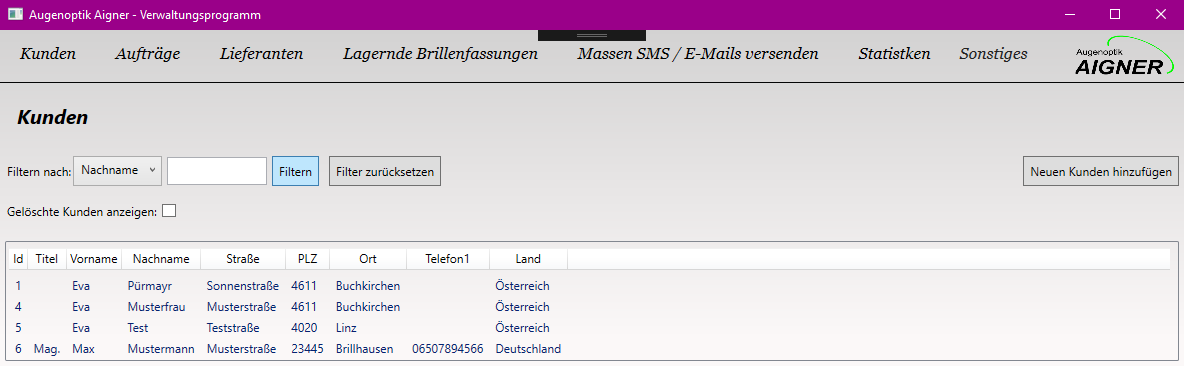
\includegraphics[scale=.45]{images/Kunden.png}
\end{center}
	\caption{Screenshot der Kundenverwaltung}
	\label{fig:sample}
\end{figure}
Beim Klick des Buttons ''Neuen Kunden hinzufügen'' erscheint ein neues Fenster, welches einen neuen Kunden erstellt. Hier kann der Benutzer weitere Daten eingeben, wie beispielsweise Hobbies, Job oder den Geburtstag. Außerdem kann der Benutzer den Ort und das Land aus einer Drop-Down-List auswählen. Falls der Ort bzw. das Land noch nicht vorhanden ist, kann der Benutzer auf den danebenliegenden Knopf drücken und einen neuen Ort/Land anlegen. 
\begin{figure}[H]
\begin{center}
	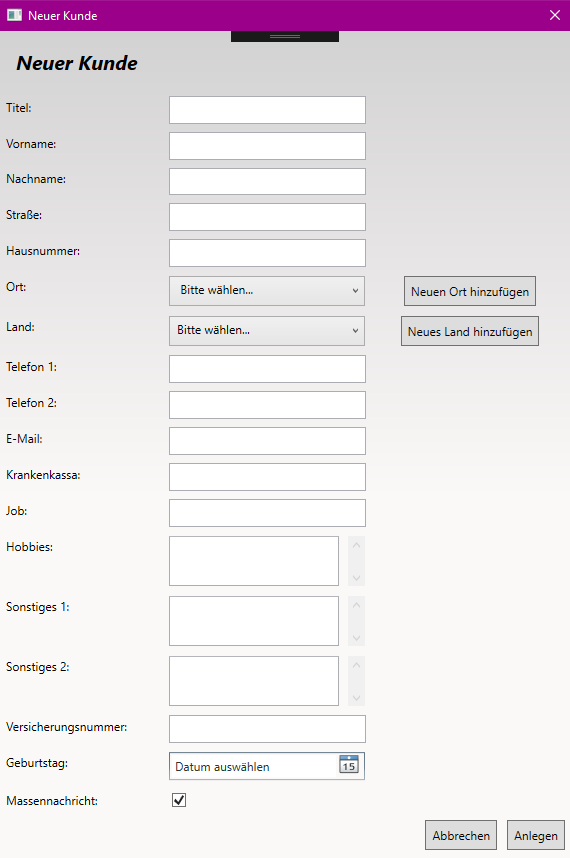
\includegraphics[scale=.3]{images/NeuerKunde.png}
\end{center}
	\caption{Screenshot Neuen Kunden anlegen}
	\label{fig:sample}
\end{figure}
Falls der Benutzer nach dem Anlegen des Kunden noch Änderungen vornehmen möchte, kann er dies auf der Startseite durch einen Doppelklick auf den gewünschten Kunden erledigen. Dadurch erscheint ein neues Fenster, auf welchem der Benutzer alle Daten des Kunden bearbeiten kann und zusätzlich alle Bestellungen des Kunden sieht. Außerdem besteht hier die Möglichkeit den Kunden zu löschen. Damit ist allerdings aus datenbanktechnischen Gründen gemeint, den Kunden nicht mehr bearbeitbar zu machen, der Benutzer kann keinen Kunden wirklich löschen. Der Grund dafür ist, dass jede Bestellung in der Datenbank auf einen Kunden verweisen muss und wenn ein Kunde bereits mehrere Bestellungen getätigt hat und der Benutzer danach den Kunden löschen möchte, würden alle seine Bestellungen mitgelöscht werden. 
\begin{figure}[H]
\begin{center}
	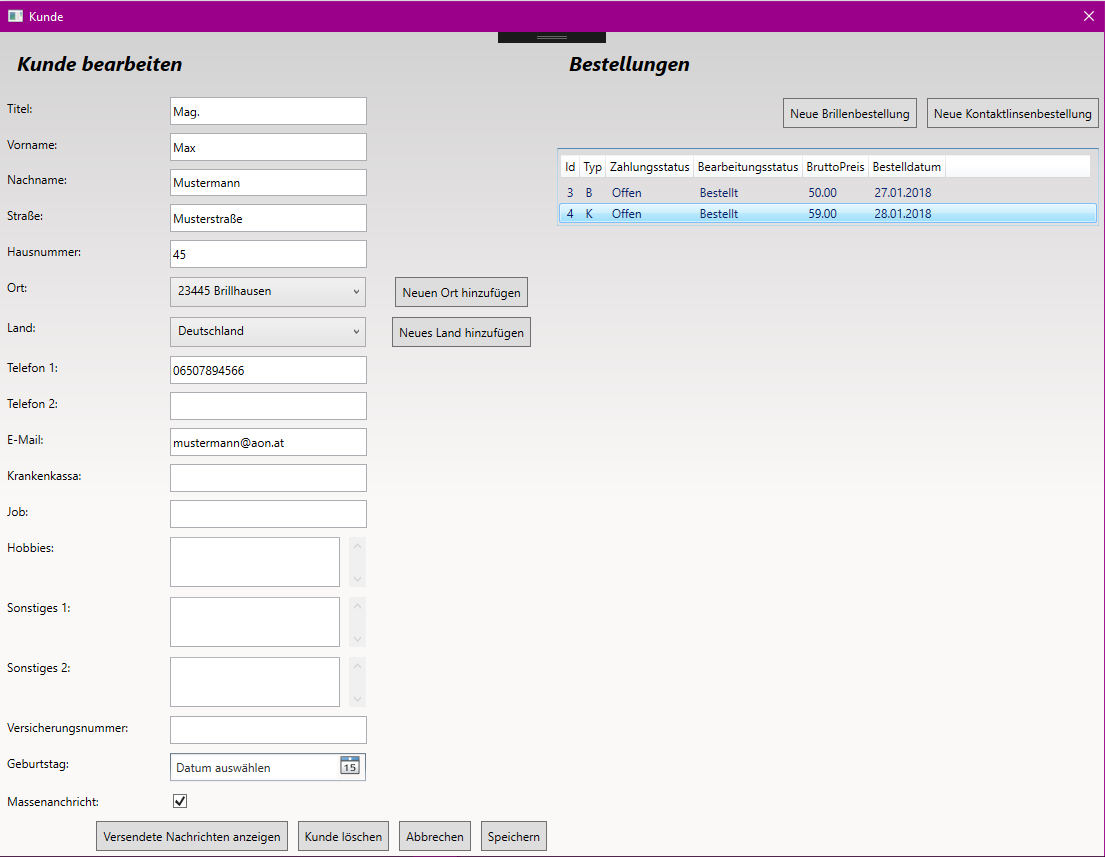
\includegraphics[scale=.25]{images/KundenDetails.png}
\end{center}
	\caption{Screenshot der Kundendetails}
	\label{fig:sample}
\end{figure}
Technischer Hintergrund:
Damit die Kunden auf der Startseite angezeigt werden können, müssen sie zuerst aus der Datenbank in eine ObservableCollection vom Typ Customer geladen werden. 
Danach wird auf Basis der Datensätze eine ICollectionView erstellt, welche die Daten dann anzeigt. Im Vergleich zur ObservableCollection bietet die ICollectionView beim Anzeigen viele Vorteile (siehe Kapitel Filtern und Sortieren). 
Um einen Kunden zu bearbeiten, muss das Objekt zuerst lokal kopiert werden.
\begin{lstlisting}
private Customer CopyCustomer(Customer item)
{
	Customer customer = new Customer();
	GenericRepository<Customer>.CopyProperties(customer, item);
	if (item.Town_Id != null)
	{
		Town town = new Town(); //Referenced town must be copied as well
		GenericRepository<Town>.CopyProperties(town, 	uow.TownRepository.GetById(item.Town_Id));
		customer.Town = town;
	}
	if (item.Country_Id != null)
	{
		Country country = new Country();
		GenericRepository<Country>.CopyProperties(country, uow.CountryRepository.GetById(item.Country_Id));
		customer.Country = country;
	}
	return customer;
}
\end{lstlisting}
Der Grund dafür ist, dass immer dieselbe Instanz von ''UnitOfWork'' verwendet wird. Wenn nur eine Referenz auf das Objekt erstellt werden würde, könnten die Änderungen nie rückgängig macht werden, weil sie ja immer sofort in die ''UnitOfWork'' übertragen werden würden.
\begin{lstlisting}
Customer cus = uow.CustomerRepository.GetById(1);
\end{lstlisting}
Beispiel: Der Benutzer öffnet einen Kunden und möchte den Vornamen von 'Max' auf 'Maxi' ändern. Bevor er die Änderung speichert, beschließt er allerdings, dass er die Änderung doch nicht vornehmen möchte und klickt statt 'Speichern' auf 'Abbrechen'. Wenn er nun auf zurück auf der Startseite ist, wurde der Vorname aber trotzdem auf 'Maxi' geändert.
Das würde passieren, wenn zuvor keine lokale Kopie erstellt worden wäre und somit der alte Vorname überschrieben worden wäre.
\newline Eine andere Möglichkeit wäre, für jeden Datenbankzugriff eine neue Instanz von ''UnitOfWork'' in einem Using-Block zu benutzen. Dann müsste man nur eine Referenz auf einen Kunden erstellen und könnte trotzdem den vorherigen Zustand wiederherstellen.
\begin{lstlisting}
using(UnitOfWork uow = new UnitOfWork())
{
	Customer cus = uow.CustomerRepository.GetById(1);
}
\end{lstlisting}
Dennoch hat auch diese Vorgehensweise Nachteile, denn dann müsste wirklich jeder einzelner Datenbankzugriff von einem Using-Block umgeben sein und das würde den Code wesentlich verlängern und unverständlicher machen.
\newline
Damit ein Kunde gelöscht werden kann, enthält die Klasse Kunde eine Property namens 'Deleted', welche angibt, ob der Kunde gelöscht wurde. Wenn diese auf 'true' gesetzt wird, kann der Benutzer den Kunden durch die Checkbox auf der Startseite ausblenden. Falls er dies nicht tut, wird der Kunde auf der Startseite angezeigt, allerdings erscheint eine Fehlermeldung, wenn der Benutzer versucht die Detailseite des Kunden zu öffnen. Dadurch ist es auch unmöglich neue Bestellungen für diesen Kunden anzulegen oder die Daten des Kunden zu bearbeiten. Die Bestellungen des gelöschten Kunden werden trotzdem normal angezeigt.
\subsection{Auftragsverwaltung}
Grundsätzlich gibt es zwei Arten von Aufträgen: Brillen- und Kontaktlinsenaufträge. Eigentlich haben beide Arten dieselben Eigenschaften, nur der Brillenauftrag verweist eine Brillenfassung und der Kontaktlinsenauftrag nicht. Außerdem hat ein Brillenauftrag einen Brillentyp und ein Kontaktlinsenauftrag einen Kontaktlinsentyp. Damit kann der Benutzer beispielsweise unterscheiden, ob es sich um eine Fern- oder Nahbrille handelt. Generell wird streng zwischen Brillen- und Kontaktlinsenaufträgen unterschieden, deshalb werden unter dem Menüpunkt ''Aufträge'' auch zwei verschiedene Listen angezeigt. Wie gewohnt kann man diese Listen wieder filtern und sortieren. Allerdings kann der Benutzer von dieser Sicht aus keine neuen Aufträge erfassen, dazu muss er in der Kundenverwaltung zuerst einen Kunden auswählen. 
\begin{figure}[H]
\begin{center}
	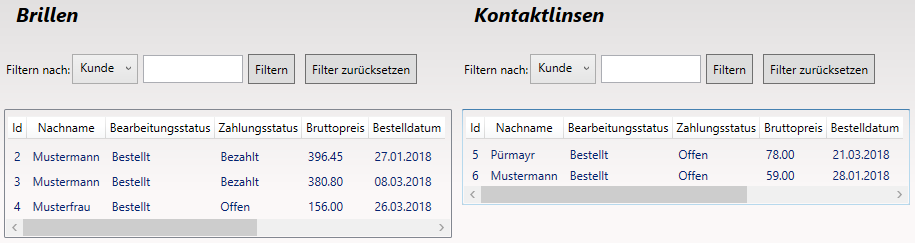
\includegraphics[scale=.45]{images/Auftraege.png}
\end{center}
	\caption{Screenshot der Auftragsverwaltung}
	\label{fig:sample}
\end{figure}
Wenn der Benutzer doppelt auf einen Auftrag klickt, erscheint entweder ein Detailfenster eines Brillenauftrags oder Kontaktlinsenauftrags. Im rechten Bereich des Fensters kann der Benutzer die einzelnen Preise der Komponenten angeben. Das Programm rechnet alle Preise  brutto und gibt zum Schluss die darin enthaltene Mehrwertsteuer an. Es wird nach folgender Formel gerechnet: Zuerst werden linker und rechter Glaspreis, Preis von Sonstigem und wenn vorhanden der Verkaufspreis der Brillenfassung addiert. Davon wird das Krankenkassageld abgezogen, der Selbstbehalt hinzugezählt und der Rabatt (dieser wird in Euro angegeben) wieder subtrahiert. Zwanzig Prozent davon sind schlussendlich die Mehrwertsteuer. 
Im unteren Bereich des Fensters kann der Benutzer Details zur Glasverarbeitung angeben. Wenn der Benutzer den Bearbeitungsstatus auf ''Abgeholt'' setzt, wird auch der Status der Brillenfassung in der Brillenfassungsverwaltung auf ''Verkauft'' gesetzt.
\begin{figure}[H]
\begin{center}
	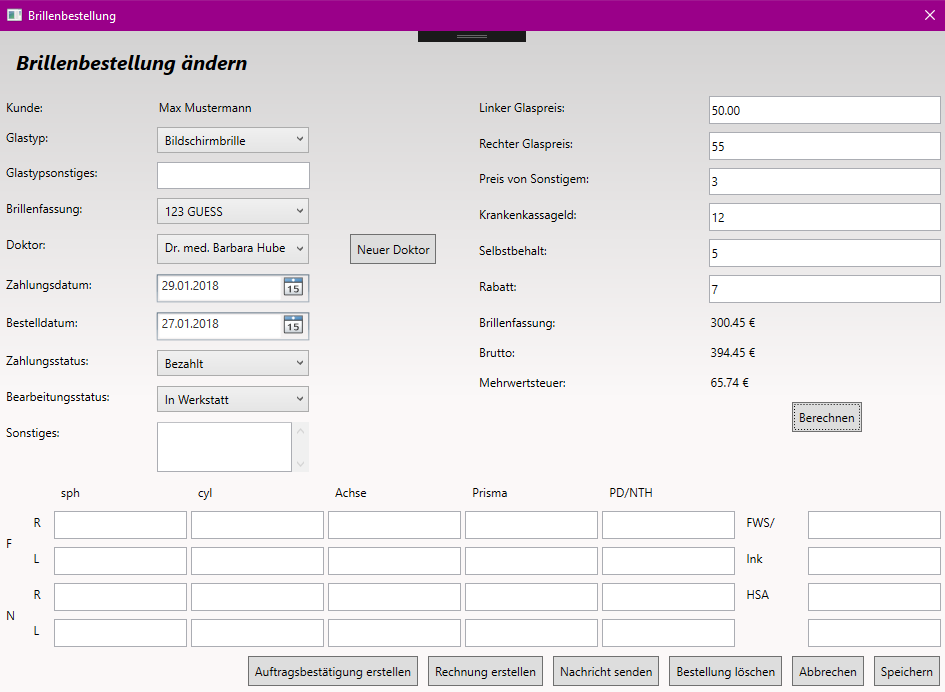
\includegraphics[scale=.3]{images/Brillenauftrag.png}
\end{center}
	\caption{Screenshot eines Brillenauftrags}
	\label{fig:sample}
\end{figure}
\subsubsection{Dokumente erstellen}
Unter den Angaben der Details zu den Gläsern, kann der Benutzer eine Auftragsbestätigung oder eine Rechnung erstellen. Die Dokumente werden als Word-Dokumente in einem Ordner abgespeichert. Das hat den Vorteil, dass der Benutzer selbst entscheiden kann, ob er noch etwas nachträglich ändern will oder das generierte Dokument gleich ausdruckt oder versendet. Gleichzeitig hat das Benutzen eines Word-Dokuments auch einen großen Nachteil, denn wenn der Benutzer nachträglich etwas ändert, wird diese Information nicht in das System weitergeleitet und somit könnten die erstellten Dokumente und der Auftrag selbst nicht dieselben Informationen beinhalten. Außerdem wird in der Datenbank immer nur der Pfad der zuletzt erstellten Rechnung/Auftragsbestätigung gespeichert. Das bedeutet, dass der Benutzer auch mehrere Dokumente zum selben Auftrag erstellen kann. Diese könnten sich auch voneinander unterscheiden, worüber das Programm ebenfalls keine Kontrolle hat. In diesem Fall wird nur ein Hinweis mit dem abgespeicherten Dokumentnamen angezeigt und gefragt ob das alte Dokument wirklich überschrieben werden soll.
\newline Damit das automatische Erstellen der Word-Dokumente funktioniert, muss der Benutzer  eine Word-Vorlage erstellen, die Felder enthält (MergeFields), welche das Programm ersetzen kann. Der Dokumentname der generierten Datei besteht immer aus der Bestell-Id, dem Dokumenttyp (Rechnung oder Auftragsbestätigung), dem Nachnamen des Kunden und dem aktuellen Datum. 
\newline Eine generierte Auftragsbestätigung könnte so aussehen:
\begin{figure}[H]
\begin{center}
	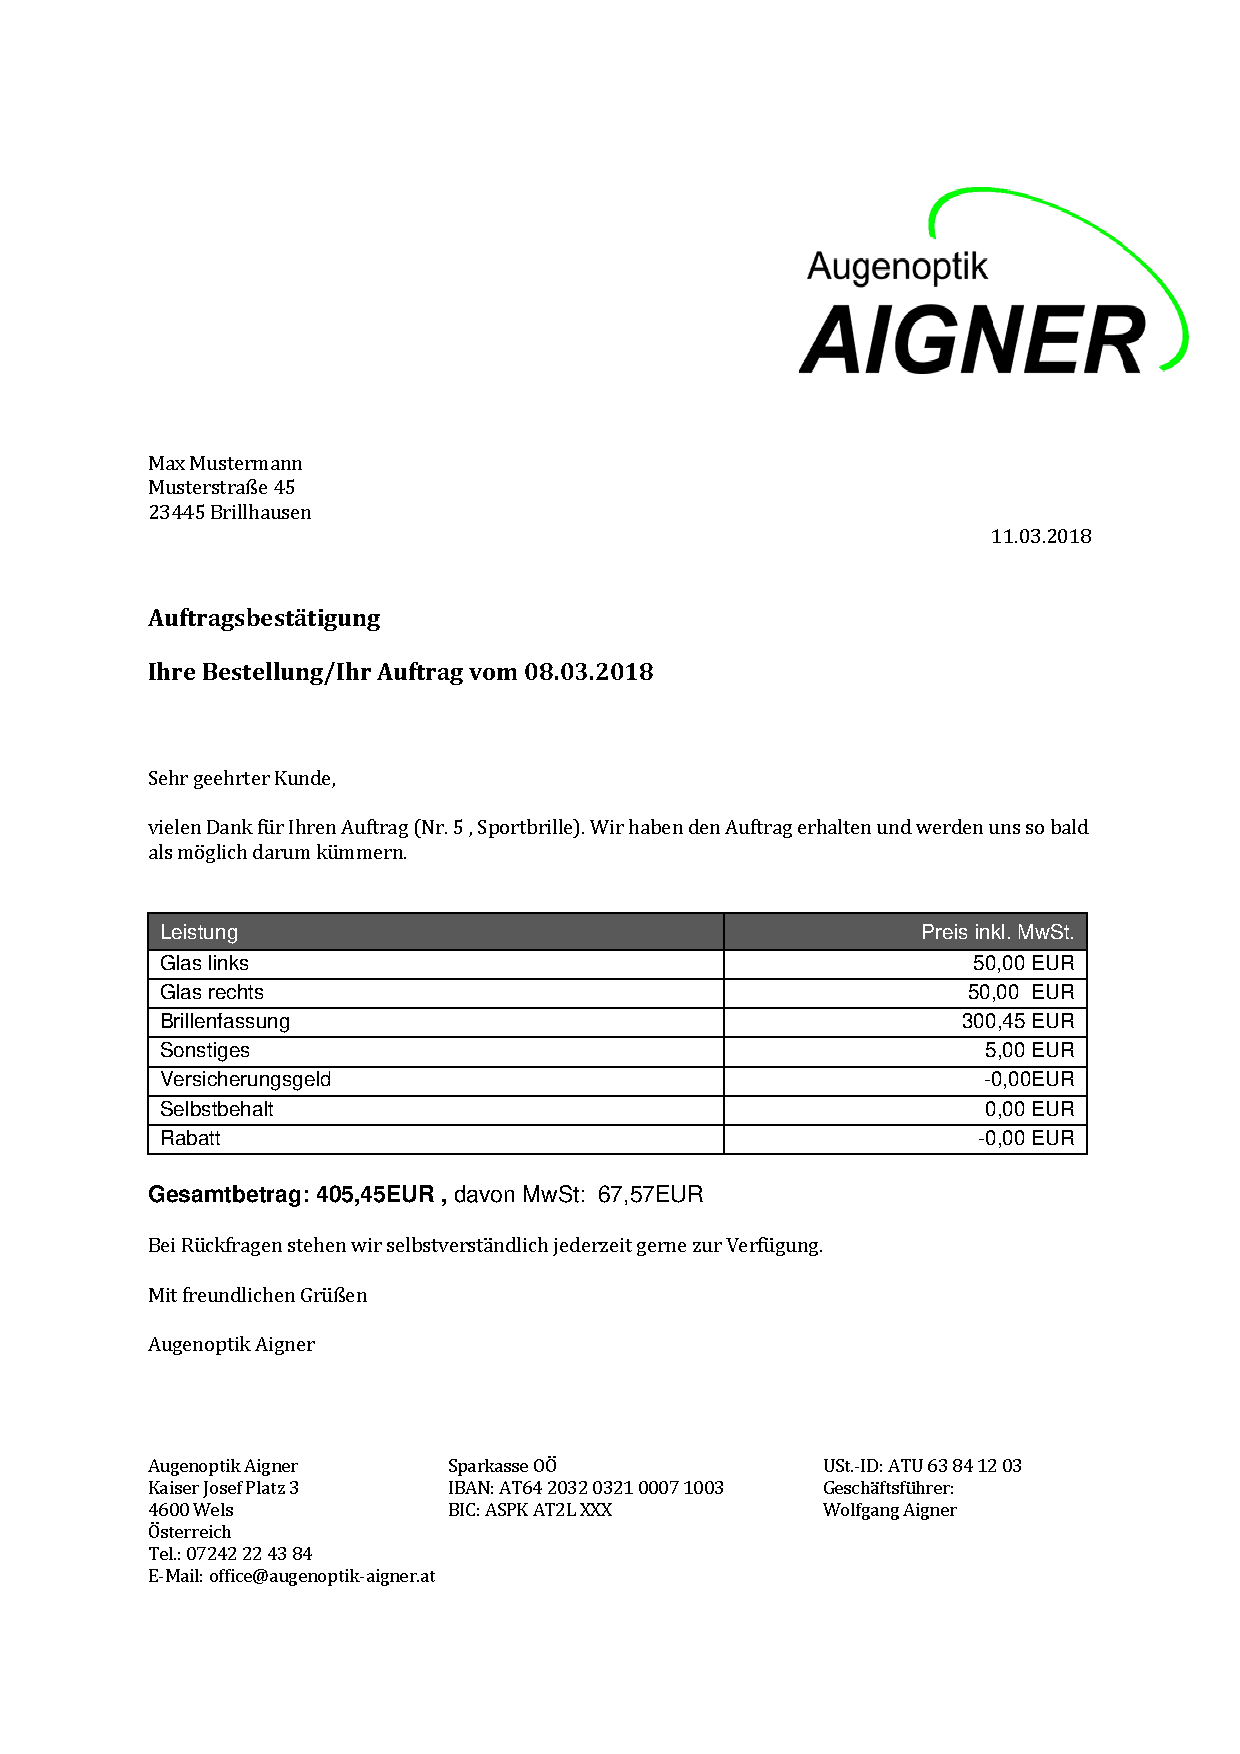
\includegraphics[scale=.75]{images/MusterAuftragsbestaetigung.pdf}
\end{center}
	\caption{Generierte Auftragsbest\"atigung}
	\label{fig:sample}
\end{figure}
Technischer Hintergrund:
Zur Erstellung von Word-Dokumenten wird Interop verwendet (siehe Kapitel 2.6). Die Methode CreateDocument benutzt eine vom Benutzer erstellte Wordvorlage und ersetzt die Mergefields. Der erste Parameter ''orderId'' gibt die Id der gewählten Bestellung an. Mit Hilfe dieser Nummer können aus der Datenbank die restlichen Daten geladen werden. Der Parameter oTemplatePath beschreibt den Pfad der Wordvorlage und der String path den Namen, unter dem das Dokument abgespeichert werden soll. Der Code unterhalb ist nur ein Ausschnitt der Methode.
\begin{lstlisting}
private static bool CreateDocument(int orderId, Object oTemplatePath, string path)
{
	Application wordApp = new Application();
	Document wordDoc = new Document();
	try
	{
		Order order;
		Customer cus;
		//Ausgeschnitten: Hier werden Order und Customer Werte aus der Datenbank zugewiesen 
		Object oMissing = System.Reflection.Missing.Value;
		wordDoc = wordApp.Documents.Add(ref oTemplatePath, ref oMissing, ref oMissing, ref oMissing);
		foreach (Field myMergeField in wordDoc.Fields)
		{
			Range rngFieldCode = myMergeField.Code;
		 	String fieldText = rngFieldCode.Text;
		 	
		 	//Nur Mergefields sollte bearbeitet werden
		 	if (fieldText.StartsWith(" MERGEFIELD")
		 	{
		 		string translatedFieldName;
		 		//Ausgeschnitten: Hier wird der Name der Property aus dem fieldText herausgeholt und auf Englisch uebersetzt
		 		string value = String.Empty;
		 		//Ausgeschnitten: Die Property wird in den Klassen gesucht und der Wert gespeichert z.B: Properties der Klasse Customer:
		 		if (typeof(Customer).GetProperty(translatedFieldName) != null)
		 		{
		 			value = cus.GetType().GetProperty(translatedFieldName).GetValue(cus, null)?.ToString();
		 		}
		 		myMergeField.Select();
		 		wordApp.Selection.TypeText(value);
		 	}
		 }
		 int idx = oTemplatePath.ToString().LastIndexOf("\\");
		 string p = oTemplatePath.ToString().Substring(0, idx + 1);
		 string completePath = p + path + ".docx";
		 wordDoc.SaveAs(completePath);
		 wordDoc.Close();
		 wordApp.Quit();
		 return true;
	}
	catch (Exception e)
	{
		Console.WriteLine(e);
		wordApp.Quit();
		wordDoc.Close();
		return false;
	}
}
\end{lstlisting}
Zuerst werden eine neue Applikation und ein neues Dokument erstellt. Nachdem der Auftrag und der Kunde aus der Datenbank geladen worden sind, wird die Vorlage für das Dokument geladen. Dabei ist nur der erste Parameter (''oTemplatePath'') von Bedeutung. Danach werden in einer Foreach-Schleife alle Felder des Dokumentes durchgegangen. Dabei werden nur jene bearbeitet, bei denen der Text des Feldes mit ''MERGEFIELD'' beginnt (es gibt auch Arten von Feldern in Word, jedoch sind in der Vorlage alle zu bearbeitenden Felder sogenannte Mergefields). Dann wird die gesuchte Property (Code ausgeschnitten) mit Hilfe der Variable ''fieldText'' ermittelt. ''fieldText'' muss aber zuerst auf Englisch übersetzt werden, da die Namen der Felder in der Vorlage deutsch sind, die Properties der Klassen aber Englisch. Der übersetzte Name der Property wird in der Variable ''translatedFieldName'' gespeichert. Anschließend werden allen Klassen nach dem Propertynamen durchsucht. Wenn die richtige Klasse gefunden wurde, wird der Wert der Property des Objekts in der Variable ''val'' gespeichert. Danach wird an Stelle des Mergefields in der Vorlage der ermittelten Wert eingetragen. Zum Schluss wird noch der gewünschte Pfad ermittelt und das Dokument unter diesem Pfad gespeichert.
Genau die selbe Methode wird benutzt, wenn eine Rechnung erstellt wird, die so aussehen könnte:
\begin{figure}[H]
\begin{center}
	\includegraphics[scale=.75]{images/Musterrechnung.pdf}
\end{center}
	\caption{Generierte Rechnung}
	\label{fig:sample}
\end{figure}
\subsection{Lieferantenverwaltung}
Ebenso wie für die Kunden, gibt es auch eine Verwaltung für die Lieferanten des Benutzers. Auch die Lieferanten lassen sich filtern und sortieren (siehe Kapitel Filtern und Sortieren). Lieferanten haben folgende Attribute: Name, Ort, Land, Adresse, FAX, Telefon, E-Mail, Kundennummer (damit ist die Id des Benutzers beim jeweiligen Lieferanten gemeint), Kontaktperson, Produkte und Sonstiges. Einen neuen Lieferant kann man mittels dem Button links oben anlegen und Lieferanten bearbeiten und löschen kann der Benutzer durch einen Doppelklick auf den gewünschten Lieferanten.
\begin{figure}[H]
\begin{center}
	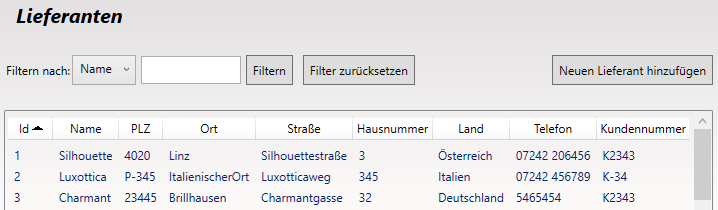
\includegraphics[scale=.45]{images/Lieferanten.png}
\end{center}
	\caption{Screenshot der Lieferantenverwaltung}
	\label{fig:sample}
\end{figure}
\subsection{Verwaltung der lagernden Brillenfassungen}
Genau wie bei der Verwaltung der Kunden und der Lieferanten gibt es auch eine Verwaltung der lagernden Brillenfassungen. Jede Brille die der Optiker verkauft, hat eine eigene Fassung und die wird hier erfasst. Dabei hat jede Brillenfassung folgende Attribute: Modell, Marke, Farbe, Größe, Status (bestellt, lagernd oder verkauft), Einkaufspreis, Einkaufsdatum, Verkaufspreis, Verkaufsdatum und der Lieferant. Die Liste kann wie gewohnt gefiltert und sortiert werden. Um eine neue Brillenfassung zu erfassen kann der Benutzer auf den Button links oben klicken und um eine bestehende Brillenfassung zu bearbeiten oder zu löschen muss der Benutzer einen Doppelklick auf die gewünschte Brillenfassung tätigen.
\newline Eigentlich würde man erwarten, dass zu den Brillenfassungen auch die Anzahl an lagernden Stück abgespeichert wird. Allerdings wurde dieses Feature nach Absprache mit dem Auftraggeber nicht implementiert, da jede Brillenfassung für jeden Auftrag einzeln bestellt wird. Deswegen wird auch der Status der Brillenfassung gespeichert.
\begin{figure}[H]
\begin{center}
	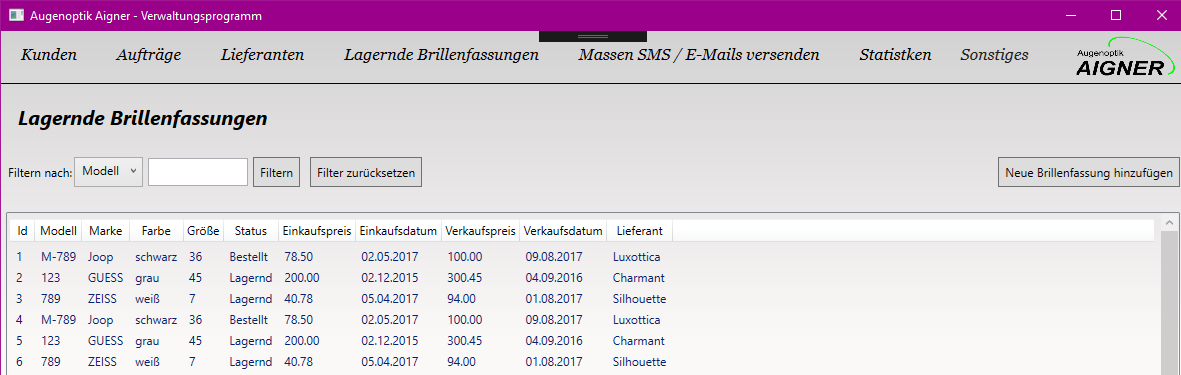
\includegraphics[scale=.45]{images/Brillenfassungen.png}
\end{center}
	\caption{Screenshot der lagernden Brillenfassungen}
	\label{fig:sample}
\end{figure}
\subsection{E-Mail und SMS}
\subsubsection{Massennachrichten}
Um regelmäßige Info- und Werbenachrichten auszusenden, bietet das Programm die Möglichkeit E-Mails oder SMS an alle Kunden zu versenden. Falls ein Kunde diese Nachrichten nicht mehr erhalten möchte, kann das der Benutzer bei dem einzelnen Kunden eintragen.
\subsubsection{E-Mail}
Wenn der Benutzer eine Massenmail versenden möchte, kann er einen Betreff und eine Nachricht eingeben, die nachher an alle Kunden gesendet wird. Als E-Mail-Adresse, wird die abgespeicherte Adresse des Kunden verwendet. Falls keine E-Mail-Adresse angegeben wurde, wird eine entsprechende Fehlermeldung angezeigt.

\begin{figure}[H]
\begin{center}
	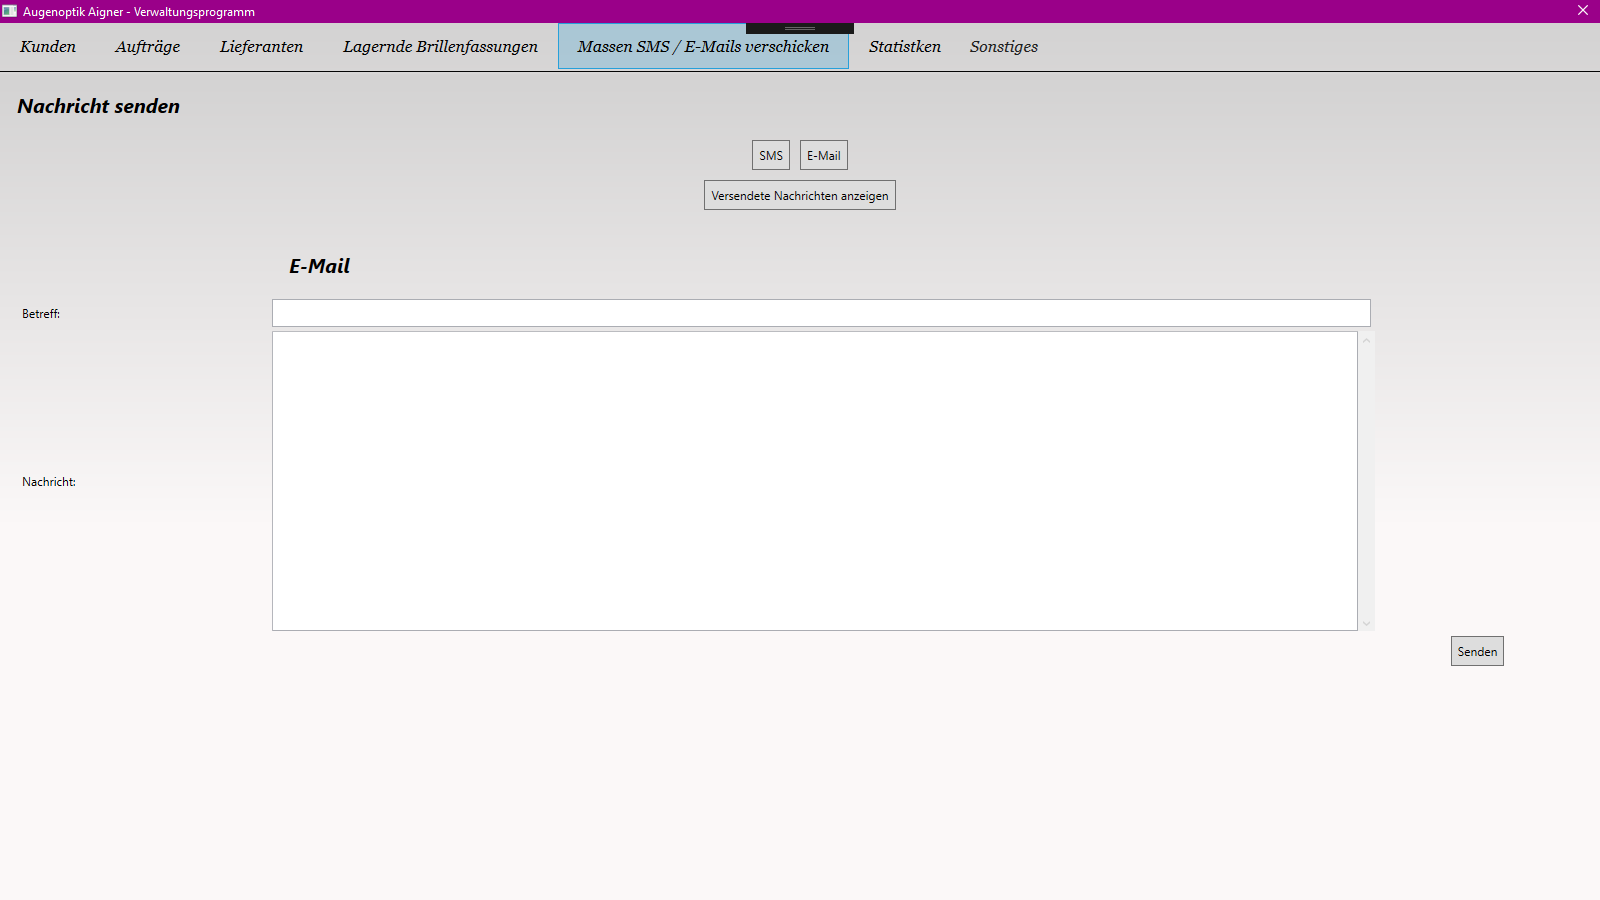
\includegraphics[scale=.4]{images/Massenemail.png}
\end{center}
	\caption{Screenshot der Massen E-Mails}
	\label{fig:sample}
\end{figure}
\underline{Technischer Hintergrund:}
\medskip
\linebreak
Es wird für jeden Kunden die gleiche Mail erstellt (Klasse MailMessage vom Namespace System.Net.Mail). Diesem Objekt werden Attribute wie Sender, Empfänger, Betreff, Nachricht usw. gesetzt und mittels eines SMTP-Clients versendet (Klasse SmtpClient ebenfalls vom Namespace System.Net.Mail). Der Smtp-Client bekommt noch Informationen wie Host, Port und natürlich die E-Mail-Adresse, von der die E-Mail weggeschickt werden soll, sowie das Passwort für die E-Mail-Adresse. In diesem Fall wurde eine Gmail-Adresse verwendet, die extra für diesen Zweck erstellt wurde.

\begin{lstlisting}
var message = new MailMessage();
message.To.Add(new MailAddress(item.Email));
message.From = new MailAddress("infodienst.augenoptikaigner@gmail.com");
message.Subject = this.Subject;
message.Body = this.Message;
this.Recipients.Add(new CustomRecipient() { Customer = item, Address = item.Email });

using (var smtp = new SmtpClient())
{
	var credential = new NetworkCredential
	{
		UserName = "infodienst.augenoptikaigner@gmail.com",
		Password = //not shown here
	};
	smtp.Credentials = credential;
	smtp.Host = "smtp.gmail.com";
	smtp.Port = 587;
	smtp.EnableSsl = true;
	await smtp.SendMailAsync(message);
}       
\end{lstlisting}
\bigskip
Danach wird die gesendete Nachricht noch in die Datenbank abgespeichert, damit der Benutzer später einen Überblick über alle gesendeten Nachrichten hat.

\subsubsection{SMS}
Zum Versenden der SMS wird der SMS-Dienst MessageBird verwendet (siehe Kapitel 2.8). Ähnlich wie beim Versenden einer E-Mail, gibt der Benutzer wieder eine Nachricht ein, allerdings kann er keine Betreff einfügen.
\begin{figure}[H]
\begin{center}
	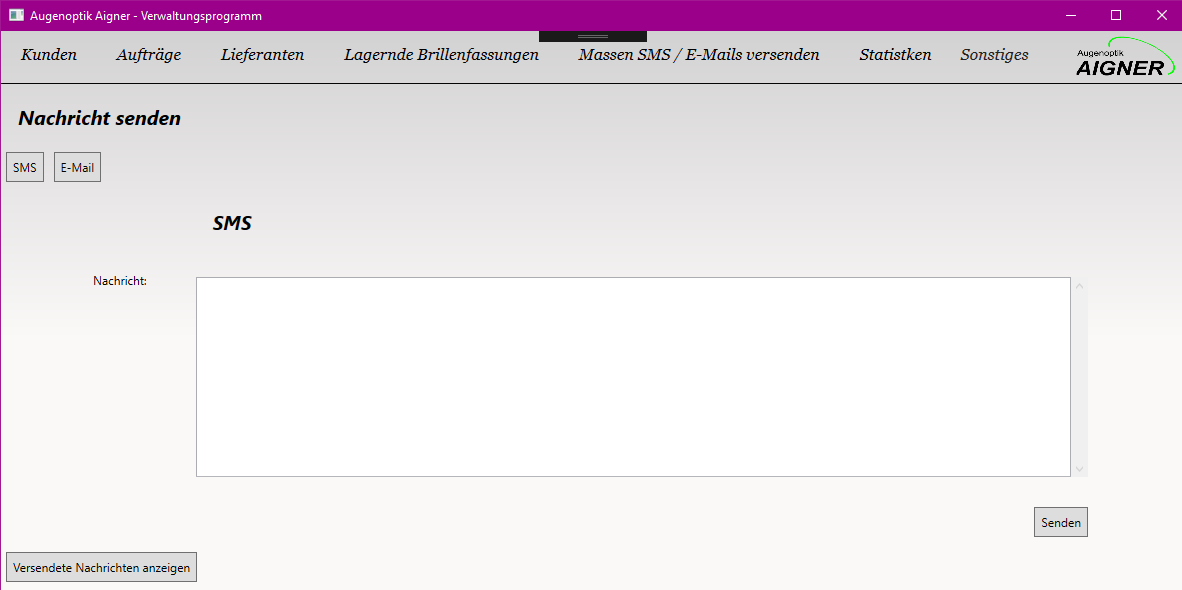
\includegraphics[scale=.4]{images/Massensms.png}
\end{center}
	\caption{Screenshot der Massen SMS}
	\label{fig:sample}
\end{figure}
Diese Nachricht wird dann an alle Kunden gesendet, außer jene, bei denen eingetragen ist, dass sie keine Massennachricht mehr erhalten wollen. Als Telefonnummer wird standardmäßig die Telefonnummer 1 gewählt, außer diese ist nicht vorhanden, dann wird die Telefonnummer 2 gewählt. Die ausgewählte Nummer sollte eine mobile Telefonnummer (kein Festnetz) sein, sonst kann die Nachricht nicht versendet werden.
\begin{comment}
\newpage
\underline{Technischer Hintergrund:}
\linebreak
\linebreak 
Zum Senden einer Nachricht werden folgende Schritte benötigt:
\begin{lstlisting}
IProxyConfigurationInjector proxyConfigurationInjector = null;
Client client = Client.CreateDefault(AccessKey, proxyConfigurationInjector);
\end{lstlisting}
Und zum Versenden einer Nachricht:
\begin{lstlisting}
MessageBird.Objects.Message message = client.SendMessage("OptikAigner", this.Message, numbers);
\end{lstlisting}
Der AccessKey ist ein normaler String, der von MessageBird erstellt wird. Dabei kann jeder Benutzer von MessageBird mehrere AccessKeys bekommen, beispielsweise einen für Test-Nachrichten, die dann nicht versendet werden oder einen Key, mit dem dann echte SMS versendet werden.
Für jede Nachricht die versendet wird, wird das Guthaben auf MessageBird dementsprechend verringert. Sollte das Guthaben auslaufen, wird eine Fehlermeldung angezeigt.
\end{comment}

\subsubsection{Einzelne Nachrichten}
Dieselben Vorgänge werden auch verwendet um einzelne Nachrichten zu versenden. Dazu muss der Benutzer auf die Detailseite einer Bestellung klicken und dann auf „Nachricht senden“. Standardmäßig wird ein Text eingefügt, der dem Kunden mitteilt, dass seine Bestellung nun abholbereit ist. Sollte dies nicht der Grund sein, warum eine Nachricht gesendet werden soll, kann der Benutzer die Nachricht natürlich auch verändern.
\begin{figure}[H]
\begin{center}
	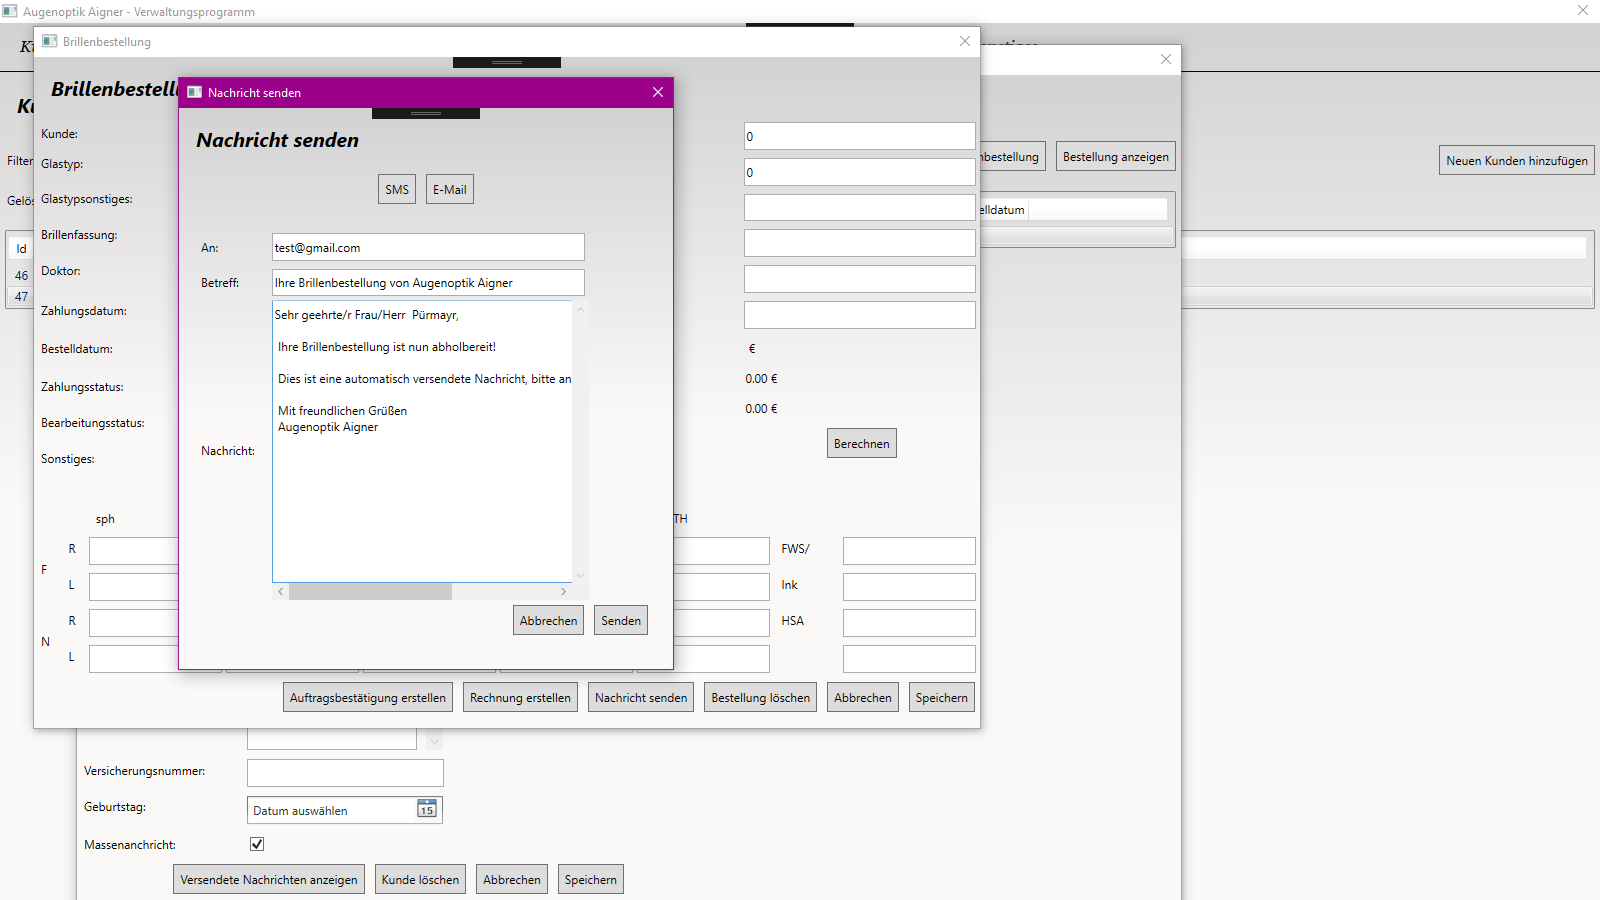
\includegraphics[scale=.4]{images/EinzelneNachricht.png}
\end{center}
	\caption{Screenshot der einzelnen Nachricht}
	\label{fig:sample}
\end{figure}
\subsubsection{Versendete Nachrichten}
Außerdem ist es möglich, alle Nachrichten, die vom System aus gesendet worden sind, anzuzeigen. Um nur Nachrichten anzuzeigen, die an einen bestimmten Kunden gesendet worden sind, muss der Benutzer auf die Detailseite eines Kunden klicken und dann die „Versendeten Nachrichten“ anzeigen. Falls der Benutzer alle Nachrichten sehen will, die er versendet hat, kann er diese unter dem Menüpunkt „Massen SMS /E-Mails verschicken“ sehen.\\
Dazu wurden in der Datenbank extra die Tabellen ''CustomMessage'' und ''CustomRecipient'' angelegt, um alle Nachrichten und deren Empfänger abspeichern zu können. Hier wird beispielsweise eine Massensms gespeichert:
\begin{lstlisting}
var m = new CustomMessage();
m.Date = DateTime.Now;
m.MessageText = this.Message;
m.MessageType = OpticiatnMgr.Core.Entities.MessageType.SMS;
m.Recipients = new List<CustomRecipient>();
var numbers = GetPhoneNumbers();
for (int i = 0; i < this.Customers.Count; i++)
{
	m.Recipients.Add(new CustomRecipient() { Customer = this.Customers[i], Address = numbers[i].ToString() });
}
uow.MessageRepository.Insert(m);
uow.Save();
\end{lstlisting}
\begin{figure}[H]
\begin{center}
	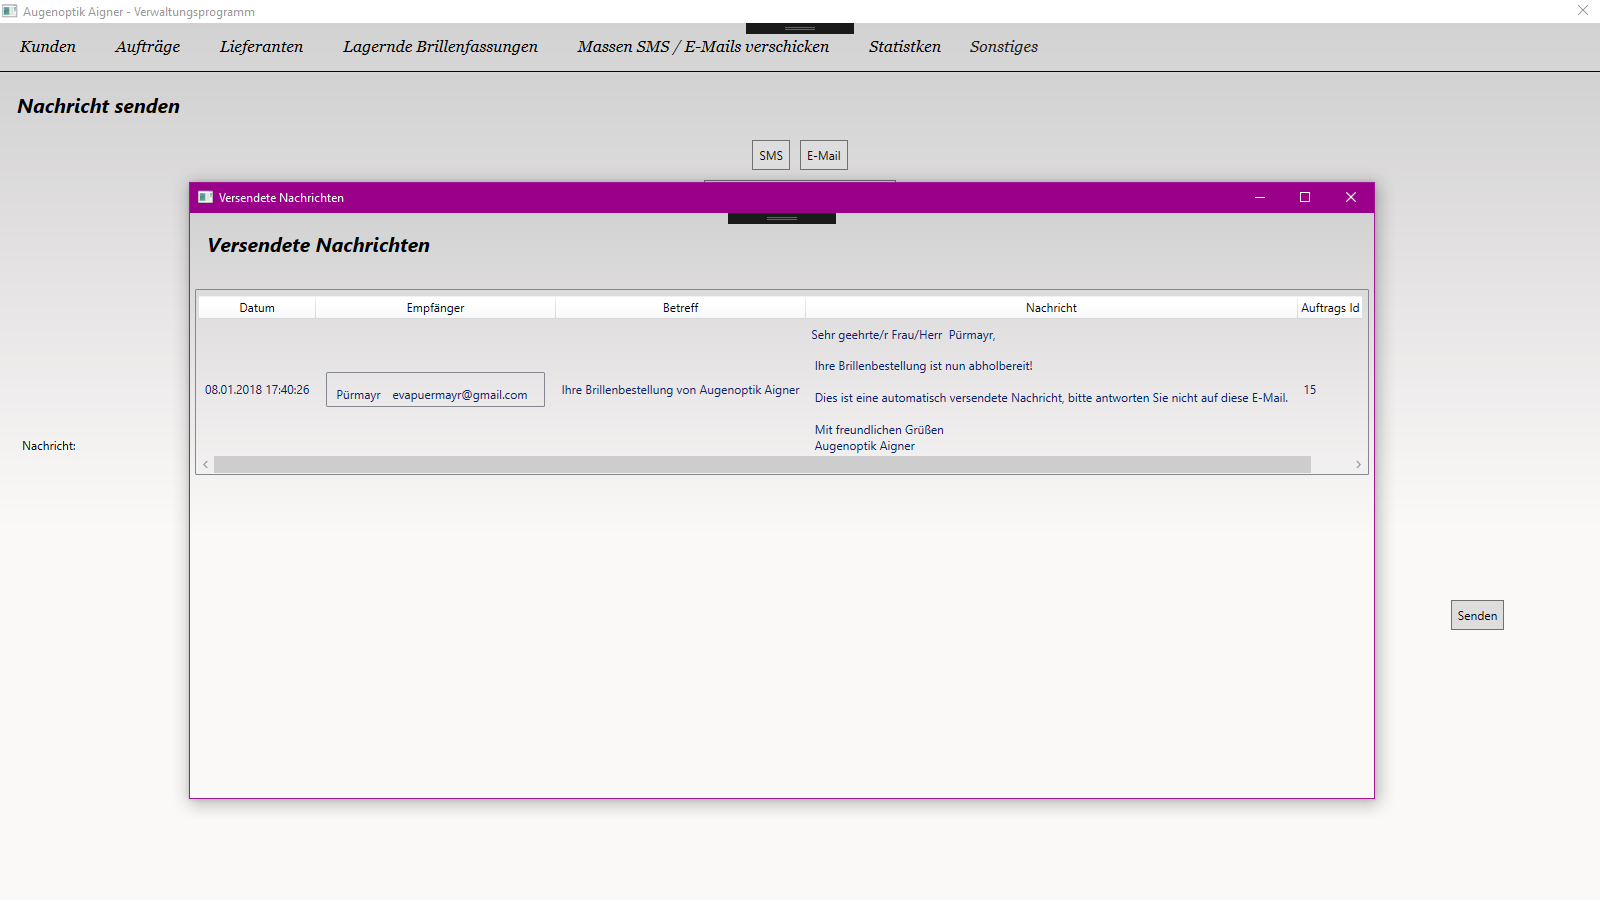
\includegraphics[scale=.5]{images/VersendeteNachrichten.png}
\end{center}
	\caption{Screenshot der versendeten Nachrichten}
	\label{fig:sample}
\end{figure}

\subsection{Statistiken}
Unter dem Menüpunkt ''Statistiken'' erhält der Benutzer eine Übersicht über alle verkauften Brillen und Kontaktlinsen. Dazu wird ein Liniendiagramm der verkauften Brillen/Kontaktlinsen von diesem Jahr und dem Jahr davor angezeigt. Damit ein Brillen/Kontaktlinsenauftrag in der Statistik mitberücksichtigt wird, muss ein Zahlungsdatum angegeben werden und der Bezahlungsstatus muss auf „Bezahlt“ gesetzt werden.
\begin{figure}[H]
\begin{center}
	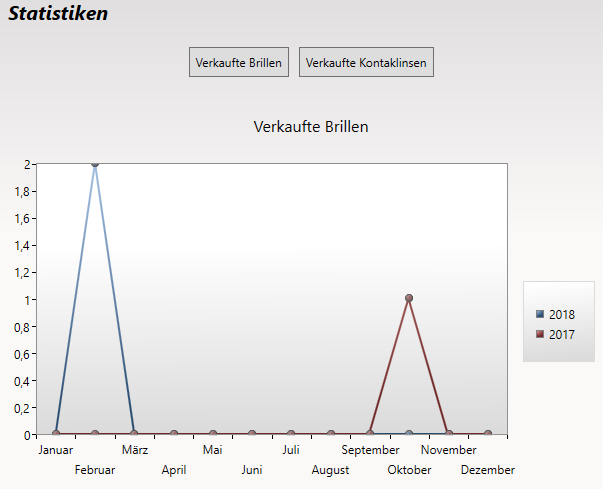
\includegraphics[scale=.4]{images/Statistiken.png}
\end{center}
	\caption{Screenshot der Statistiken}
	\label{fig:sample}
\end{figure}
\subsubsection{Technischer Hintergrund}
Zur Darstellung wurde das Wpf-Toolkit verwendet (siehe Kapitel 2.7).
\begin{comment} 
Dazu wird in dem .xaml File der Namespace angegeben: 
\begin{lstlisting}
<Page xmlns:toolkitCharting="clr-namespace:System.Windows.Controls
DataVisualization.Charting;assembly=System.Windows.Controls.DataVisualization
.Toolkit">
\end{lstlisting}
\end{comment}
Um ein Liniendiagramm zu erzeugen:
\begin{lstlisting}
<toolkitCharting:Chart Title="{Binding Title}">
            <toolkitCharting:LineSeries Title="{Binding NewYear}"  DependentValueBinding="{Binding Value}" IndependentValueBinding="{Binding Key}" ItemsSource="{Binding NewValues}"/>
            <toolkitCharting:LineSeries Title="{Binding OldYear}"  DependentValueBinding="{Binding Value}" IndependentValueBinding="{Binding Key}" ItemsSource="{Binding OldValues}"/>
</toolkitCharting:Chart>
\end{lstlisting}
Dabei sind ''NewValues'' und ''OldValues'' vom Typ: 
\begin{lstlisting}
public ObservableCollection<KeyValuePair<string, int>> NewValues { get; set; }
public ObservableCollection<KeyValuePair<string, int>> OldValues { get; set; }
\end{lstlisting}
Die Daten werden mittels Linq (Kapitel 2.1.1) erfasst.
\subsection{Sonstiges}
Unter dem Menüpunkt ''Sonstiges'' erscheinen vier Unterpunkte: 
\begin{itemize}
\item Orte bearbeiten
\item Länder bearbeiten
\item Brillentypen bearbeiten
\item Kontaktlinsentypen bearbeiten
\end{itemize}
Wie die Überschriften schon vermuten lassen, öffnen diese vier Buttons jeweils ein eigenes Fenster, welches eine Übersicht über alle vorhandenen Objekte zeigt. Am Beispiel ''Länder'' wird nun die Verwendung gezeigt:
\begin{figure}[H]
\begin{center}
	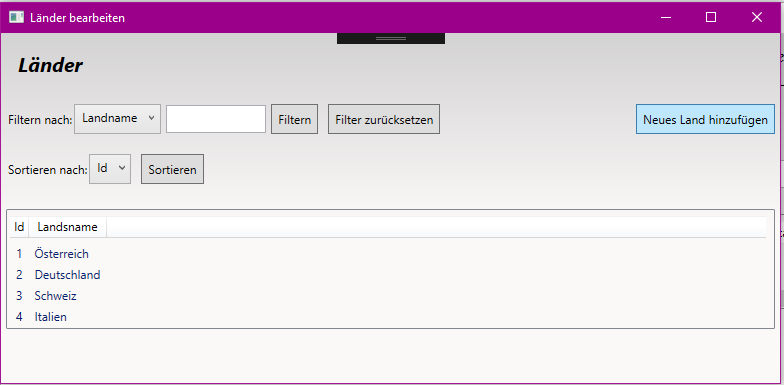
\includegraphics[scale=0.75]{images/Laender.png}
\end{center}
	\caption{Screenshot der L\"ander}
	\label{fig:sample}
\end{figure} 
Im oberen Bereich können die Länder nach Name oder Id gefiltert werden. Allerdings funktioniert das Sortieren hier anders als bei den Übersichtlisten. Der Benutzer kann auswählen, nach was er gerne sortieren möchte und danach sortiert das Programm aufsteigend nur nach dieser einen Property. Mit einem Doppelklick kann ein Land bearbeitet/gelöscht werden und rechts oben kann ein neues Land hinzugefügt werden.
\begin{figure}[H]
\begin{center}
	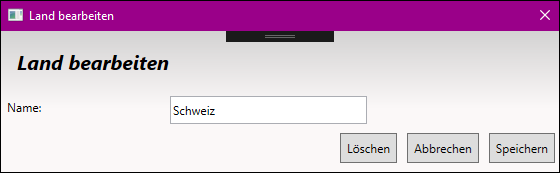
\includegraphics[scale=0.75]{images/LandBearbeiten.png}
\end{center}
	\caption{Land bearbeiten}
	\label{fig:sample}
\end{figure} 
\subsection{Filtern und Sortieren}
\subsubsection{Filtern}
Auf allen Hauptseiten der Applikation (Kunden, Brillen- und Kontaktlinsenaufträge, Lieferanten, Lagernde Brillenfassungen) sowie auf den Seiten unter dem Menüpunkt „Sonstiges“ (Orte, Länder, Brillen- und Kontaktlinsentypen) ist es möglich die Datensätze zu filtern. Dies passiert immer nach demselben Schema, dennoch ist diese Funktion für jede dieser Seiten einzeln implementiert.
Dazu muss der Benutzer das Feld aussuchen, nach welchem er gerne filtern möchte, danach einen Text eingeben und dann auf „Filtern“  oder die Taste „Enter“ drücken. Das Programm gibt nun nur jene Datensätze aus, bei denen das gewünschte Feld den eingegebenen Text enthält. Neben dem „Filtern“-Button befindet sich ein „Filter löschen“-Button, der wieder alle Datensätze zum Vorschein bringt.
\begin{figure}[H]
\begin{center}
	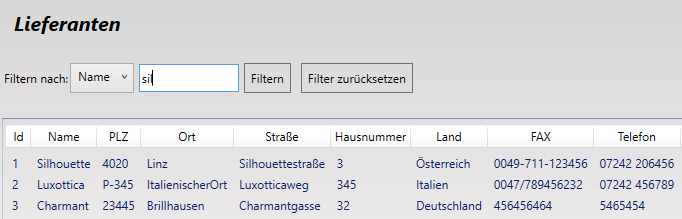
\includegraphics[scale=0.75]{images/filter.png}
\end{center}
	\caption{Screenshot des Filters}
	\label{fig:sample}
\end{figure}
Im nachfolgenden Beispiel wird anhand der „Lagernden Brillenfassungen“ erklärt wie der Filter funktioniert. 
Im ViewModel gibt es ein Feld, welches ''PropertiesList'' heißt (vom Typ ObservableCollection\textless string\textgreater). In diesem werden alle Felder der jeweiligen Klasse aufgezählt. Davor werden noch Felder, nach denen der Benutzer später nicht filtern sollte, herausgestrichen. Bei Referenzen auf andere Objekte, zum Beispiel bei der Brillenfassung der Lieferant, wird die ''Supplier\_Id'' entfernt, der String ''Supplier'' bleibt allerdings in der Liste. Später beim Übersetzen in Englisch wird überprüft, ob nach einem Fremdschlüssel gefiltert wird. In diesem Fall wird der Name des Fremdschlüssels (hier ''Supplier'') zu dem Hauptnamen in der Property umgewandelt (''SupplierName''). Das bedeutet, dass wenn der Lieferant als Filterfeld ausgewählt wird, in Wirklichkeit nur nach einem Feld (hier dem Namen des Lieferanten) gefiltert wird.
\newline Nachdem aller Felder ausgewählt wurden, wird jedes Feld in Deutsch übersetzt. Dies geschieht mittels einem kleinen Wörterbuch (Klasse ResourceManager), welches eine Übersetzung für jedes Feld bereithält. Die Wörter, die im ResourceManager stehen, müssen selbst eingefügt werden und werden in einem File namens ''Resources.resx'' unter den Properties des Projektes abgespeichert. Neben einfachen Wörtern könnten hier auch Bilder, Dateien oder Ähnliches verwaltet werden. Hier wird die Liste der Felder aus denen der Benutzer später sein „Filterfeld“ auswählen kann erstellt. 
\begin{lstlisting}
public ObservableCollection<String> PropertiesList { get; }

private ResourceManager manager = Properties.Resources.ResourceManager;

private ObservableCollection<string> GetAllProperties()
{
	ObservableCollection<string> props = new 							ObservableCollection<string>(typeof(EyeGlassFrame).GetProperties()
.Select(p => p.Name).ToList());
	ObservableCollection<string> newList = new ObservableCollection<string>();
	props.Remove("Timestamp"); //Shouldnt be able to filter by timestamp
   props.Remove("Supplier_Id"); //Shouldnt be able to filter by supplier_id
   foreach (var item in props)
   {
   		var germanItem = manager.GetString(item);
   		if (germanItem != null)
             newList.Add(germanItem);
   }
   return newList;
}
\end{lstlisting}
Wenn der Benutzer einen Text eingibt und danach „Filtern“ drückt, wird das Feld, das er gewählt hat zuerst mit Hilfe des ResourceManagers auf Englisch übersetzt.  Danach wird die Methode Filter() aufgerufen, die den passenden Filter setzt, falls der Benutzer einen Text eingegeben hat.
\begin{lstlisting}
public void Filter()
{
	try
	{
		if (!String.IsNullOrEmpty(this.FilterText))
		{
			this.EyeGlassFramesView.Filter = new Predicate<object>(Contains);
		}
		else
			this.EyeGlassFramesView.Filter = null;
	}
	catch (Exception e)
	{
		Console.WriteLine(e.StackTrace);
	}
}
\end{lstlisting}
Dabei muss man wissen, dass EyeGlassFramesView vom Typ ICollectionView ist. Diese Property wird im Konstruktor aus der Liste der wirklichen Brillenfassungen erzeugt (EyeGlassFrames). Der Typ ICollectionView ist als Anzeigeelement für Listen gedacht, weshalb es auch ein Feld namens „Filter“ gibt. Durch die Methode „Contains“ wird dieser auch gesetzt. Der folgende Code stammt aus dem ViewModel der lagernden Brillenfassung.
Properties:
\begin{lstlisting}
public ObservableCollection<EyeGlassFrame> EyeGlassFrames { get; set; }
public ICollectionView EyeGlassFramesView { get; set; }
public string TranslatedFilterProperty { get; set; }
public string FilterText { get; set; }
\end{lstlisting}
Im Konstruktor wird EyeGlassFramesView initialisiert.
\begin{lstlisting}
this.EyeGlassFramesView = CollectionViewSource.GetDefaultView(EyeGlassFrames);
\end{lstlisting}
Die Methode Contains gibt zurück, ob das Objekt „f“ dem angegebenen Filter entspricht. Dazu wird zunächst überprüft, ob die Klasse EyeGlassFrame die Property enthält, nach der der Benutzer filtert. Wenn ja, gibt die Methode zurück, ob in dieser Property die Zeichenkette vorkommt, nach der der Benutzer sucht. Danach überprüft das Programm ob die gesuchte Eigenschaft eine Eigenschaft der Klasse Supplier ist. Das passiert, weil jede lagernde Brillenfassung einen Lieferanten hat. Deswegen kann es sein, dass der Benutzer nach einer Eigenschaft filtert, die gar nicht in der Klasse EyeGlassFrame enthalten ist, sondern nur in der Klasse Supplier. Wenn keiner dieser Fälle zutrifft, was nicht vorkommen sollte, wird eine Fehlermeldung zurückgegeben.
\begin{lstlisting}
private bool Contains(object f)
{
	EyeGlassFrame frame = f as EyeGlassFrame;
	if (typeof(EyeGlassFrame).GetProperty(TranslatedFilterProperty) != null)
	{
		return frame.GetType().GetProperty(this.TranslatedFilterProperty)
		.GetValue(frame, null)?.ToString().ToUpper().IndexOf(this.FilterText.ToUpper()) >= 0;
	}
	else if (typeof(Supplier).GetProperty(TranslatedFilterProperty) != null) //Does the user filter by suppliername?
	{
		return frame.Supplier?.GetType()
		.GetProperty(this.TranslatedFilterProperty)
		.GetValue(frame.Supplier, null)?.ToString().ToUpper().IndexOf(this.FilterText.ToUpper()) >= 0;
	}
	else
	{
		MessageBox.Show("Beim Filtern ist ein Fehler aufgetreten!");
		return false;
	}
}
\end{lstlisting}
\subsubsection{Sortieren}
Bei den allen Hauptseiten, auf denen Daten angezeigt werden, ist eine dynamische Sortierung implementiert. Diese macht es dem Benutzer möglich, nach drei Spalten gleichzeitig auf- oder absteigend zu sortieren.  Dazu muss der Benutzer auf eine beliebige Spaltenüberschrift klicken. Das ist dann die Spalte, nach der zuerst aufsteigend sortiert wird. Drückt der Benutzer erneut auf dieselbe Spaltenübersicht, werden die Datensätze nach dieser Spalte absteigend sortiert. Wenn der Benutzer nach einer zweiten Spalte sortieren möchte, muss er zusätzlich die Shift-Taste drücken, während er die Spaltenüberschrift auswählt. Wiederrum muss der Benutzer ein zweites Mal mit der Shift-Taste die gleiche Spaltenüberschrift anklicken, um absteigend zu sortieren. Dasselbe gilt für die dritte Spalte. Um die Sortierung wieder zurücksetzen zu können, kann der Benutzer eine andere Spaltenüberschrift mit einem normalen Klick wieder sortieren. Im nachfolgenden Bild hat der Benutzer zuerst nach dem Vornamen, dann nach Ort und zum Schluss nach Nachnamen sortiert. Zur besseren Übersichtlichkeit zeigt das Programm einen normalen Pfeil oder einen Pfeil mit einem oder zwei Punkten, je nachdem in welcher Reihenfolge die Spalten sortiert wurden.
\begin{figure}[H]
\begin{center}
	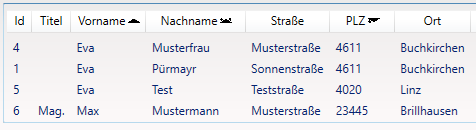
\includegraphics[scale=0.75]{images/Sortieren.png}
\end{center}
	\caption{Screenshot des Sortierens}
	\label{fig:sample}
\end{figure}
Zur Implementierung gibt es eine Klasse SortManager, die die Sortierung für alle Hauptseiten regelt.
\begin{lstlisting}
public SortManager SortManager { get; set; }
\end{lstlisting} 
Dazu wird im Konstruktor ein neuer SortManager initialisiert.
\begin{lstlisting}
SortManager = new SortManager();
\end{lstlisting}
Zusätzlich werden drei Events von der View abonniert. Dieses Event wird von der ListView bereitgestellt.
\begin{lstlisting}
<i:Interaction.Triggers>
	<i:EventTrigger EventName="Loaded">
		<cmd:EventToCommand Command="{Binding Initialized}"
                                        PassEventArgsToCommand="True" />
	</i:EventTrigger>
</i:Interaction.Triggers>
\end{lstlisting}
In jedem ListViewHeader werden noch Shift+LeftClick und MouseDown abonniert.
\begin{lstlisting}
<GridViewColumn DisplayMemberBinding="{Binding FirstName, UpdateSourceTrigger=PropertyChanged}">
	<GridViewColumnHeader Content="Vorname">
		<GridViewColumnHeader.InputBindings>
			<MouseBinding Gesture="Shift+LeftClick" Command="{Binding SortShift}" CommandParameter="FirstName" >
			</MouseBinding>
		</GridViewColumnHeader.InputBindings>
		<i:Interaction.Triggers>
			<i:EventTrigger EventName="MouseDown">
				<cmd:EventToCommand Command="{Binding SortCommand}"
                                        PassEventArgsToCommand="True" />
			</i:EventTrigger>
		</i:Interaction.Triggers>
	</GridViewColumnHeader>
</GridViewColumn>
\end{lstlisting}
Im ViewModel gibt es die zugehörigen ICommands:
\begin{lstlisting}
public ICommand SortCommand { get; set; }
public ICommand SortShift { get; set; }
public ICommand Initialized { get; set; }
\end{lstlisting}
Diese werden im Konstruktor initialisiert:
\begin{lstlisting}
SortCommand = new RelayCommand<RoutedEventArgs>(SortS);
SortShift = new RelayCommand<object>(SortSh);
Initialized = new RelayCommand<RoutedEventArgs>(Init);
\end{lstlisting}
Im ViewModel werden dann folgende Methoden aufgerufen:
\begin{lstlisting}
private void Init(RoutedEventArgs p)
{
	SortManager.Init(p);
}
//Click without shift key
private void SortS(RoutedEventArgs e)
{
	var tmp = this.CustomersView;
	SortManager.SortNormal(e, ref tmp);
}
//Click with shift
private void SortSh(object p)
{
	var tmp = CustomersView;
	SortManager.SortShift(p, ref tmp);
}
\end{lstlisting}
In der Methode SortManager.Init(RoutedEventArgs p) werden durch die Variable p alle GridViewColumnHeader abgespeichert. Der Grund dafür ist, dass bei dem Event SortShift keine EventArgs mitgegeben werden können, weil es sich um ein MouseBinding handelt und nicht um ein normales Event. Dadurch kann die Methode SortShift(object p, ref ICollectionView View) nicht wissen, welche Spaltenüberschrift gedrückt wurde und daher müssen am Anfang einmal alle GridViewColumnHeaders abgespeichert werden.
Wenn die Methode SortNormal(RoutedEventArgs e, ref ICollectionView View) aufgerufen wird, wird zunächst überprüft ob die Spaltenüberschrift schon einmal gedrückt wurde (dann soll nämlich die Sortierrichtung geändert werden). Wenn ja, werden die Suchrichtung sowie die Richtung des Pfeils neben der Spaltenüberschrift geändert. Ansonsten werden alle Pfeile neben den Überschriften gelöscht, die Suchrichtung auf aufsteigend gesetzt und ein neuer Pfeil gesetzt. Ein Auszug der SortNormal-Methode:
\begin{lstlisting}
//Same column pressed?
if (SortHeaders.Count == 1 && SortHeaders[0] == columnHeader)
{
	//Change sort direction
	dir = View.SortDescriptions[0].Direction;
	dir = dir == ListSortDirection.Ascending ? ListSortDirection.Descending : ListSortDirection.Ascending;
	header = ChangeArrow(columnHeader, dir, 0);
}
else
{
	//Remove arrow from old column header
	if (SortHeaders.Count > 0)
	{
		foreach (var item in SortHeaders)
		{
			item.Column.HeaderTemplate = null;
			item.Column.Width = item.ActualWidth - 20;
		}
	}
	SortHeaders.Clear();
	SortHeaders.Add(columnHeader);
	//default sort direction is ascending
	dir = ListSortDirection.Ascending;
	header = SetNewArrow(columnHeader, dir, 0);
}
View.SortDescriptions.Clear();
View.SortDescriptions.Add(new SortDescription(header, dir));
\end{lstlisting}
SortHeaders ist eine globale Variable vom Typ List\textless GridViewColumnHeader\textgreater , der die Spalten enthält, nach welchen aktuell sortiert wird. Die lokale Variable ''dir'' bezeichnet die gewünschte Sortierrichtung und ist vom Typ ListSortDirection. Der String ''header'' enthält die Property, auf die der GridViewColumnHeader bindet. Diese ist natürlich Englisch und stellt wieder ein Übersetzungsproblem dar. \newline Wie schon weiter oben erwähnt, ist der Typ ICollectionView extra für das Darstellen von Listen gemacht, deshalb enthält er auch eine Eigenschaft SortDescriptions, in welche man beliebig viele SortDescriptions einfügen kann und nach welchen die Liste automatisch sortiert wird. In den Methoden ChangeArrow und SetNewArrow wird die Spalte entsprechend breiter gemacht und das passende vorgefertigte Template gesetzt.
\begin{lstlisting}
column.Column.HeaderTemplate = Application.Current.FindResource("ArrowUp") as DataTemplate;
\end{lstlisting}
In diesem Beispiel wird dem GridViewColumnHeader column ein Pfeil der nach oben ausgerichtet ist beigefügt.
In der Methode SortShift(object p, ref ICollectionView View) wird mittels dem Parameter p der Name der Property übergeben, an die sich die Spalte bindet. Dieser wird händisch in der View übergeben (siehe oben) und ist englisch, weshalb er zuerst übersetzt werden muss. Danach wird der passende GridViewColumnHeader nach der Überschrift in den am Anfang angelegten GridViewColumnHeaders gesucht.

\begin{lstlisting}
var columnHeader = AllHeaders.Where(h => String.Equals(h.Content.ToString(), germanColumnName)).ToList().FirstOrDefault();
\end{lstlisting}
Dann wird wieder überprüft, ob dieselbe Spalte zweimal hintereinander ausgewählt wurde, sodass dann die Sortierrichtung gewechselt werden kann. Ansonsten wird überprüft ob schon drei Spalten ausgewählt wurden und wenn nicht wird eine neue Spalte zu den Sortierspalten hinzugefügt.
Auszug der SortShift-Methode:

\begin{lstlisting}
if (View.SortDescriptions.Count >= 1)
{
	ListSortDirection dir;
	int index = View.SortDescriptions.Count - 1;
	//Change sorting direction
	if (View.SortDescriptions.Count == index + 1 && View.SortDescriptions[index].PropertyName == columnName)
	{
		dir = View.SortDescriptions[index].Direction;
		dir = dir == ListSortDirection.Ascending ? ListSortDirection.Descending : ListSortDirection.Ascending;
		View.SortDescriptions.RemoveAt(index);
		View.SortDescriptions.Insert(index, new SortDescription(columnName, dir));
		ChangeArrow(columnHeader, dir, index);
		SortHeaders.Add(columnHeader);
	}
	else if (View.SortDescriptions.Count(s => s.PropertyName == columnName) == 0)
	{
	if (View.SortDescriptions.Count >= 3)
	{
		MessageBox.Show("Sie koennen maximal nach drei Spalten sortieren!", "Hinweis", MessageBoxButton.OK, MessageBoxImage.Exclamation);
		return;
	}
	dir = ListSortDirection.Ascending;
	SetNewArrow(columnHeader, dir, index+1);
	View.SortDescriptions.Add(new SortDescription(columnName, dir));
	SortHeaders.Add(columnHeader);
}
\end{lstlisting}
\section{Datenmodell}
\section{Projektarchitektur}